%!TEX root = ../dissertation.tex
\chapter{Introduction}
\label{introduction}
\graphicspath{{./figures/introduction/}}

\newthought{We do not have to learn language from scratch with every new person we meet.} A native of Chicago can try out a coffee shop in San Francisco without needing to laboriously work out with the barista a brand-new way of ordering an `espresso,' and a 21st century reader can largely make sense of a 19th century novel without any personal contact with its author. This degree of stability across geography and time makes language indispensable for coordination in a social species: everyone who belongs to a language community assumes that others will share at least some common beliefs, or \emph{global conventions}, about what words mean \cite{Lewis69_Convention}. In this sense, the ability to competently generalize to novel communicative partners in novel contexts is what it means to be fluent in a language.

At the same time, no two speakers of a language share exactly the same lexicon, and to make matters worse, speakers seem to constantly come up with new expressions and senses on the fly \cite{Davidson86_DerangementOfEpitaphs, Clark98_CommunalLexicons}. Drop into any conversation between friends and you’ll be wading in a stream of shorthand, lingo, slang, references, and inside jokes --- some of which you might understand, but the rest of which may be meaningful to them alone. While it is tempting to think of word meanings as residing only in dictionaries, we instead find ourselves continually negotiating new meanings for old words to communicate complex thoughts, intentions, and beliefs in context. Across repeated interactions with a particular partner or group or partners, we build up intricate, idiosyncratic models: not just about how \emph{we} as English speakers collectively use language, but how \emph{this person} is expected to use language. We learn the contours of their speech and form \emph{local conventions} from our shared history. Complex stories or ideas that took long discursive conversations to initially cover can be referred back to using a brief turn of phrase. Most strikingly, this adaptation can take place to different degrees over any time-scale: from years of close scientific collaboration to a few minutes in a doctor's office.

A core puzzle for cognitive science, then, is reconciling the overarching stability of our linguistic representations with our remarkable flexibility in coordinating on new meanings. 
What do we do when our global conventions aren't sufficient --- when we have to talk about something we've never had to talk about before with a partner we've never met? 
How do we adapt so quickly? 
And how do we determine which learned meanings we can expect to stably generalize to new contexts or partners, and which only hold in the narrow scope of one partner?

To address this puzzle, we begin by breaking down the computational challenge of coordinating on meaning into three distinct cognitive mechanisms.
While this dissertation will primarily focus on the second of these mechanisms, we will argue that all three are tightly intertwined in supporting the stability and flexibility of communication.
\begin{enumerate}
\item \textbf{Prior expectations:} When we first encounter a new communication partner in a new context, we call upon some representation about what we think different signals mean to them. This representation of meaning must be sensitive to the overall statistics of the population: more people are familiar with the use of \emph{dog} to refer to the beloved pet than \emph{sclerotic aorta} to refer to the potentially dangerous health condition. It must also be sensitive to the immediate context of the interaction: a cardiologist should have different expectations about a novel colleague than a novel patient.
\item \textbf{Rapid adaptation:} Within a few minutes of conversation, we can considerably strengthen our expectations about our partner's lexicon based on earlier utterances and feedback, and adjust our own usage accordingly. For example, even if we are not initially familiar with the term \emph{sclerotic aorta}, a few minutes spent discussing the condition in simpler terms should make us more confident using the term with that partner in the future. This social learning mechanism must allow for signal \emph{reduction} -- simpler, more efficient ways of referring to the same thing over time -- and \emph{path-dependence}: early reinforcement of certain meanings increases their later usage, however arbitrary or provisional they began. 
\item \textbf{Generalization:} When we encounter the same partner in a new context, we should expect some `stickiness' from previous learning. Language does not reset at context boundaries. In addition, the lexical model we've learned within a conversation should be largely \emph{partner-specific}. Just because we now expect Partner A to be familiar with a \emph{sclerotic aorta} shouldn't radically change our expectations about Partner B. Over enough interactions with different language users, however, our initial representations should be able to shift to take these data into account. To generalize appropriately, we must be able to correctly attribute whether a usage is idiosyncratic to a particular speaker, or a global convention we should expect to hold across the whole community.
\end{enumerate}

In the remainder of Chapter 1, we consider the empirical evidence supporting the role each of these three core competencies, reinterpret this evidence from a computational perspective, and discuss several broader implications. 
Though more wide-ranging sources of data could potentially be relevant, we restrict our present scope to a family of interactive communication experiments called \emph{repeated reference games} that will be used extensively in subsequent chapters. 
This task provides a natural and productive paradigm for studying how people coordinate on meaning in the lab. 

\section{Using repeated reference games to study convention formation in the lab}

\begin{figure*}[t!]
\centering
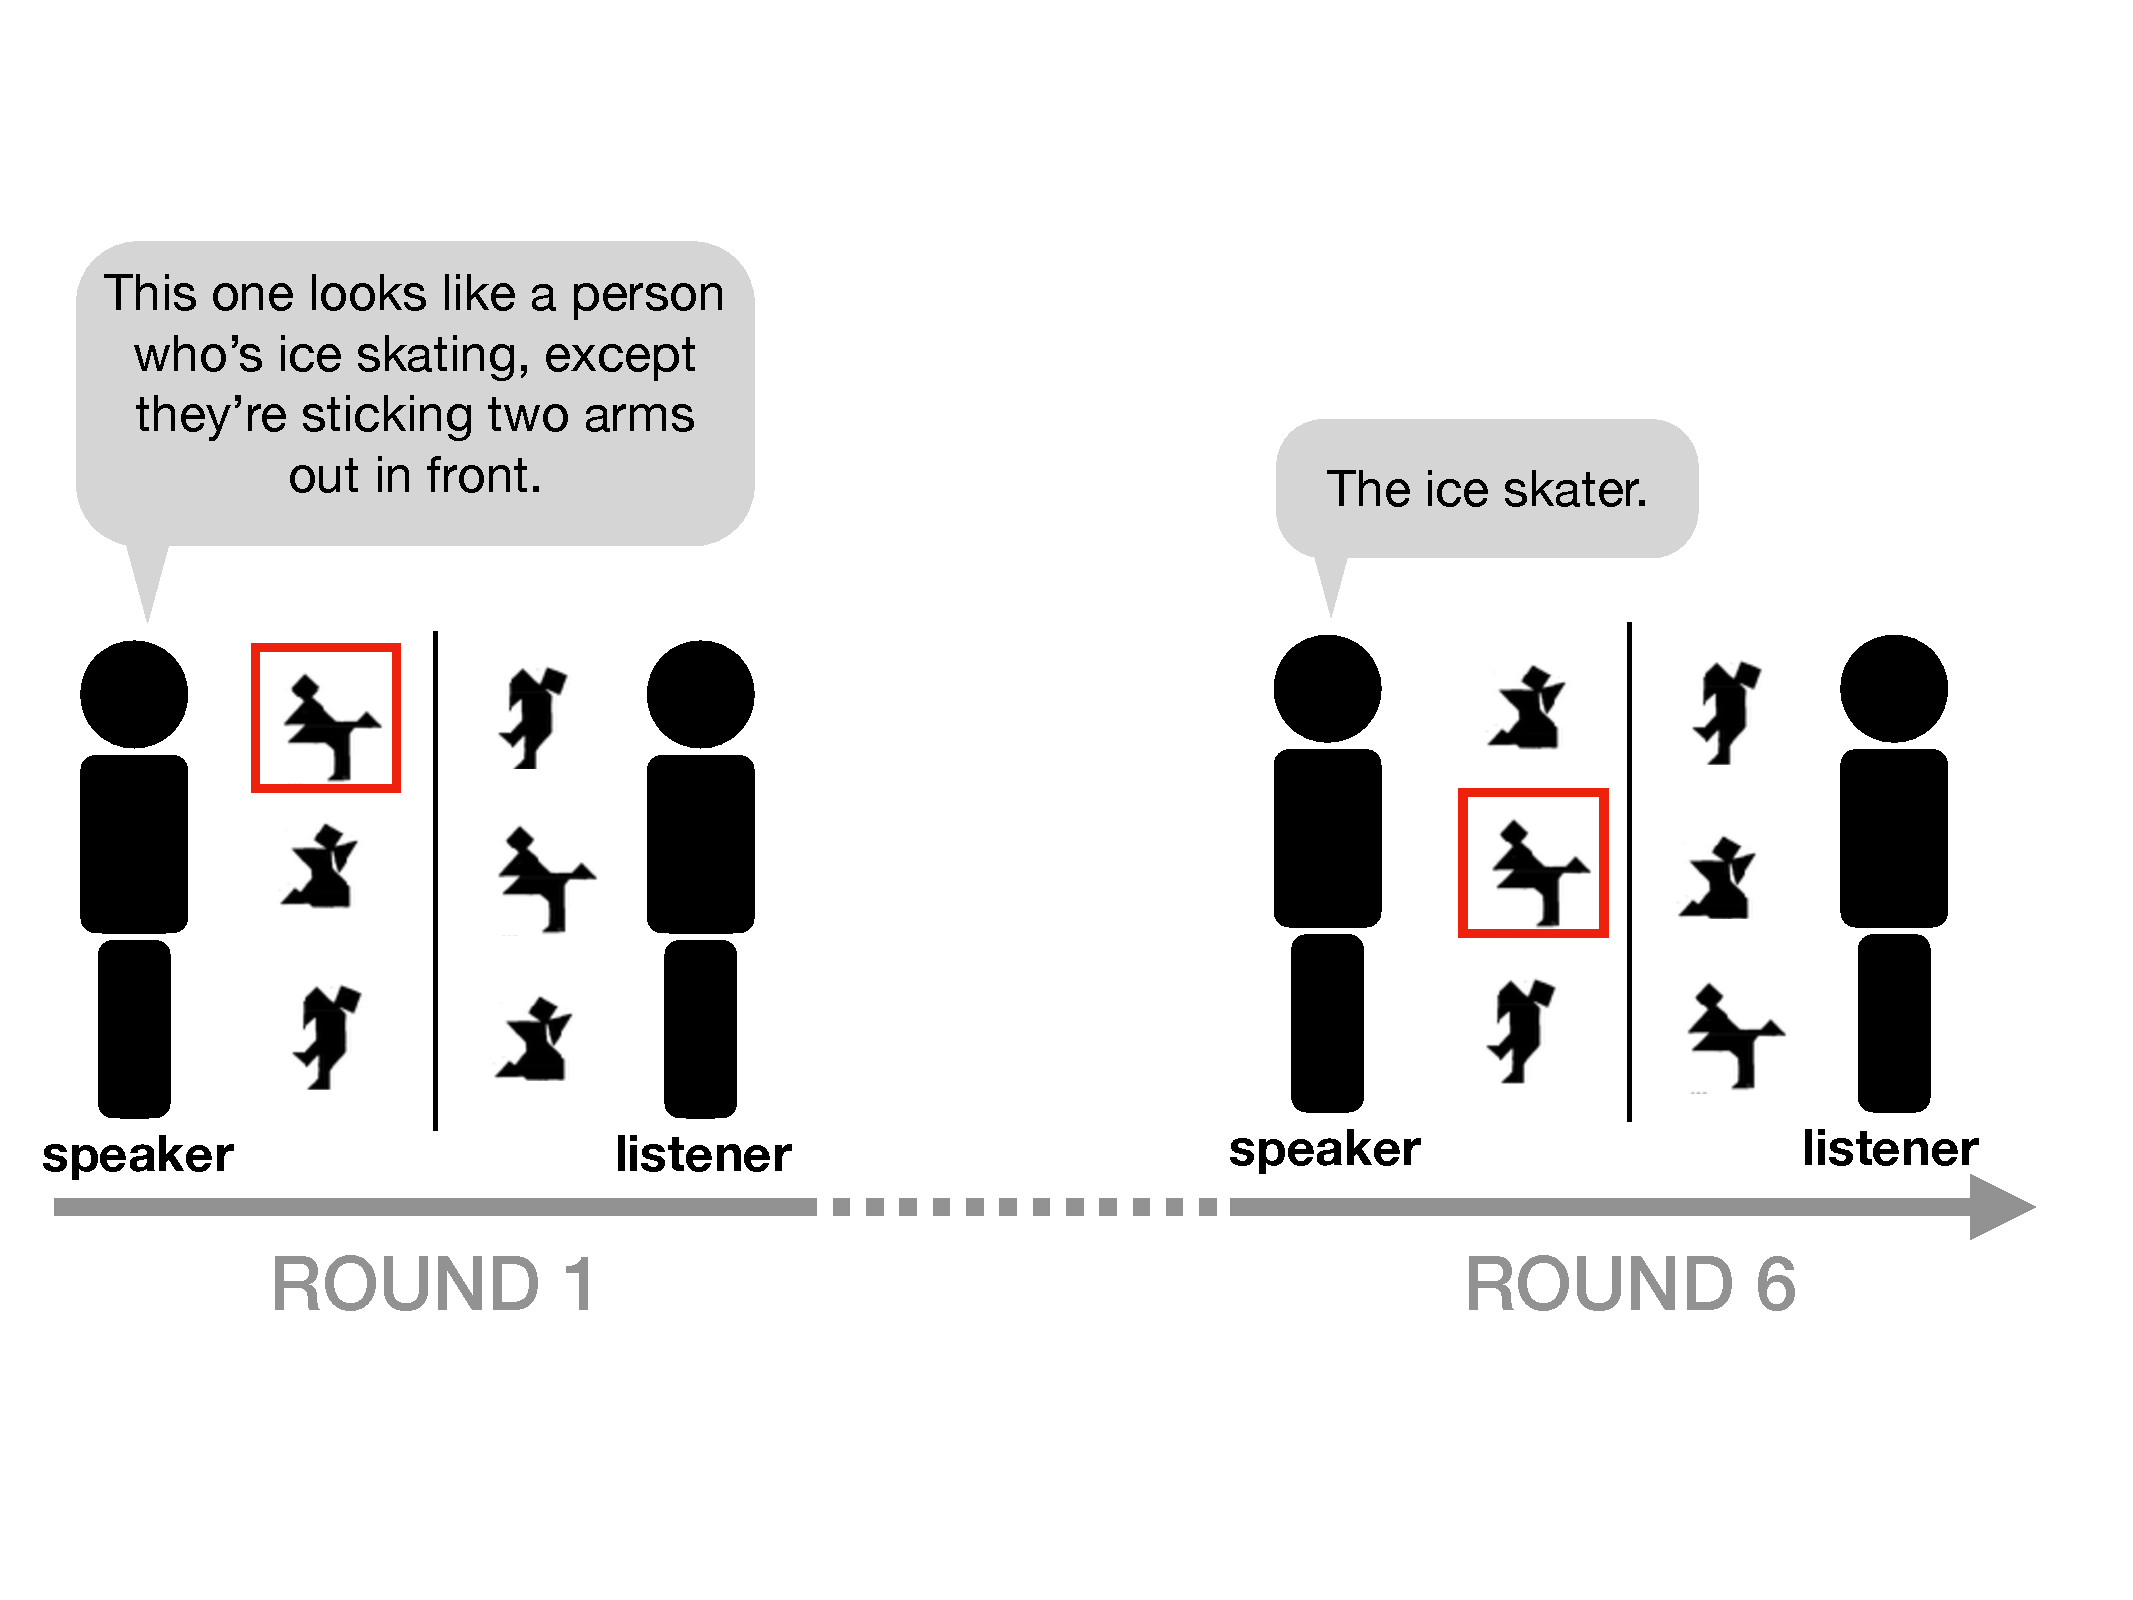
\includegraphics[scale=.43]{task_cropped.pdf}
\caption{Generic setup for repeated reference game task in the lab using stimuli from Wilkes-Gibbs \& Clark (1986); on every round, the speaker refers to each target in some context, and the listener attempts to pick out the intended referent. Both players are free to speak at any time.}
\label{fig:example}
\end{figure*}

In their simplest design (see Fig. \ref{fig:example}), pairs of participants are shown arrays of objects, presented in randomized order. On each round of the game, one player -- the speaker -- must produce a message allowing their partner to select a given target from the context. By fixing a closed set of referents and a clear communicative goal in common ground, these games vastly simplify the tangle of real-world communicative behavior. At the same time, by allowing real social partners to freely interact using natural language, we avoid the hazards of artificial or confederate-based language tasks \cite{KuhlenBrennan13_LanguageInDialogue} and expose the rich dynamics of language use in context. Given the current state of the field, then, reference games are arguably an ideal compromise between analytic tractability and ecological validity. 

% Please add the following required packages to your document preamble:
% \usepackage{booktabs}
% \usepackage{multirow}
% \usepackage{graphicx}
\begin{table}[th!]
\centering
\resizebox{\textwidth}{!}{%
\begin{tabular}{@{}lll@{}}
\toprule
\textbf{}                                   & \textbf{Parameter}                                              & \multicolumn{1}{l}{\textbf{Example parameter settings}}                 \\ \midrule
\multirow{11}{*}{\textbf{Partner design}}    & \multirow{3}{*}{What feedback is provided?}                & - no feedback at all                                                  \\
                                            &                                                                 & - only correct/incorrect                                                   \\
                                            &                                                                 & - real-time responses from partner                                         \\ \cmidrule(l){2-3} 
                                            & \multirow{3}{*}{Are you playing with the same partner?}         & - same partner for whole game                                              \\
                                            &                                                                 & - swap out partners every round                                            \\
                                            &                                                                 & - swap after $k$ rounds                                                    \\ \cmidrule(l){2-3} 
                                            & \multirow{3}{*}{What do you know about your partner?}         & - anonymous stranger                                              \\
                                            &                                                                 & - stranger with perceptual information                                            \\
                                            &                                                                 & - close friend                                                    \\ \cmidrule(l){2-3}                                             
                                            & \multirow{2}{*}{How consistent are roles across repetitions?}   & - consistent director/matcher                                              \\
                                            &                                                                 & - alternate roles each round                                               \\ \midrule
\multirow{7}{*}{\textbf{Stimulus design}}   & \multirow{2}{*}{How familiar are targets?}                      & - very familiar: colors, household objects                                 \\
                                            &                                                                 & - not at all familiar: tangrams, novel line drawings                       \\ \cmidrule(l){2-3} 
                                            & \multirow{2}{*}{How complex are targets?}                       & - very complex: busy visual scenes, clips of music                         \\
                                            &                                                                 & - not at all complex: geometric drawings                                   \\ \cmidrule(l){2-3} 
                                            & \multirow{3}{*}{How consistent are targets across repetitions?} & - exact same image of object                                               \\
                                            &                                                                 & - different pose/view of same object                                       \\
                                            &                                                                 & - different objects from same neighborhood                                 \\ \midrule
\multirow{5}{*}{\textbf{Context design}}    & \multirow{2}{*}{How similar are distractors to the target?}     & - very similar: same basic-level category                                  \\
                                            &                                                                 & - not at all similar: other categories                                     \\ \cmidrule(l){2-3} 
                                            & What is the size of context?                                    & - between 2 and 21                                                         \\ \cmidrule(l){2-3} 
                                            & \multirow{2}{*}{How consistent is context across repetitions?}  & - exact same context each round                                            \\
                                            &                                                                 & - randomized context (sometimes far, sometimes close)                      \\ \midrule
\multirow{3}{*}{\textbf{Repetition design}} & How many repetitions per target?                                & - between 3 and 100                                                        \\ \cmidrule(l){2-3} 
                                            & \multirow{2}{*}{What is spacing between repetitions?}           & - block structure                                                          \\
                                            &                                                                 & - sequential structure with interspersed contexts                          \\ \midrule
\textbf{Modality design}                    & What medium is used for communication?                          & \begin{tabular}[c]{@{}l@{}}- text\\ - audio\\ - gesture\\ - drawing\end{tabular} \\ \bottomrule
\end{tabular}%
}
\caption{\normalfont{Proposed parameterization for repeated reference games, each of which theoretically impacts the formation of conventions.}}
\label{table:parameters}
\end{table}

While one-shot reference games, which manipulate context, have been instrumental in revealing systematic pragmatic effects in the referring expressions people tend to generate \cite{KraussWeinheimer67_ReferentSimilarity,KoolenGattGoudbeekKrahmer11_Overspecification,GrafEtAl16_BasicLevel,VanDeemter16_ComputationalModelsOfReferring}, a range of even richer phenomena begin to emerge when the communication task is \emph{repeated} and the same target must be referred to multiple times. Since \citeA{KraussWeinheimer64_ReferencePhrases} first attempted such a design, many variations on this basic setup have been designed to test the boundaries of adaptation, manipulating the kinds of objects used as targets, the contexts in which the objects appear, the identity of one's partner across repetitions, the feedback available, and the medium participants use to communicate. In Table \ref{table:parameters}, we propose a potential parameterization of this family of repeated reference games, suggesting a set of conditions controlling when conventions may form. We organize our review of this literature along the three core challenges observed earlier, which roughly correspond to the temporal structure of a repeated reference game. In experimental terms: What influences the content of initial messages, how do these messages change over the coarse of the game, and under what conditions do these changes transfer to other scenarios?   %  In Table \ref{table:experiments}, we summarize 

%\todo[inline]{Provide another table summarizing a bunch of studies? Or add a column to Table 1?}

%This review is  organized around a meta-analytic parameterization of the paradigm (see Table 1), highlighting several properties of the task that appear to affect the rate at which conventions form. We then briefly contrast our hierarchical model with several different theories of adaptation and convention formation. 

\section{Mechanism \#1: A probabilistic lexicon}

People know a lot of words \cite{BergelsonAslin17_Lexicon}. Exactly how flexible knowledge about words and their meanings is structured and accessed in one's own ``mental lexicon'' remains a significant open question in cognitive science \cite{JonesEtAl15_SemanticMemory,GriffithsSteyversTenenbaum07_Topics,HuthEtAl16_SemanticMaps,GoodmanLassiter14_Semantics}. For the purpose of communicating with another speaker, however, a more relevant question is what lexicon we think our \emph{partner} is using. In this section, we review evidence from the initial rounds of repeated reference games that these lexical expectations are \emph{probabilistic} and \emph{context-sensitive}, thus providing a basis for interpreting expectations about a novel partner's lexicon as a probabilistic prior $P(\mathcal{L}_i | \Theta_0)$. 

%While a full review of ``audience design'' in generating referring expressions is outside the scope of this paper, a handful of results are directly relevant for understanding the initial lexical priors that participants bring to bear in repeated games. 

\subsection{Uncertainty in lexical expectations}

While it is convenient to view the lexicon as fixed knowledge  \cite{Cruse86_LexicalSemantics,Pinker95_LanguageInstinct,FrankGoodman12_PragmaticReasoningLanguageGames}, meanings are in reality quite flexible and ad hoc \cite{Clark83_NonceSense,ClarkGerrig83_OldWordsNewMeanings,ClarkClark79_NounsSurfaceAsVerbs,GerrigBortfeld99_SenseCreation,LascaridesCopestake98_PragmaticsWordMeaning,Glucksberg01_FigurativeLanguage,LassiterGoodman15_AdjectivalVagueness}. 
Correspondingly, recent computational models have explored the possibility that we instead represent semantic \emph{uncertainty} over which meanings our partner might intend \cite<e.g.>{CooperEtAl15_ProbabilisticTypeTheory,BergenLevyGoodman16_LexicalUncertainty,SmithGoodmanFrank13_RecursivePragmaticReasoningNIPS,PottsEtAl16_EmbeddedImplicatures,HawkinsFrankGoodman17_ConventionFormation}. 
This uncertainty leaves its signature on the initial round of repeated references games, when speakers are attempting to produce descriptions of potentially ambiguous objects for a novel partner.

In one direct demonstration, \citeA{FussellKrauss89_IntendedAudienceCommonGround} asked forty students to produce referring expressions for abstract line drawings in a repeated reference game set-up. Instead of proceeding to play the game in person, however, participants were told that their messages were intended for later identification \cite<see>[for earlier variations on this design]{KraussEtAl68_InnerSpeech, Danks70_EncodingCommunication, Innes76_InnerExternal}. Half the participants were told that these messages were intended for \emph{themselves} in the future (the `non-social' or `familiar listener' condition) while the other half were told that an anonymous other would see them (the `social' or `unfamiliar listener' condition). 

Because both groups were faced with the same communicative task, this manipulation provided some evidence about how lexical expectations differ depending on the listener. If participants used the same fixed meaning when reasoning about themselves and others, we would expect similar messages. Instead, utterances intended for others were more than twice as long as utterances for oneself (12.7 vs. 5.0 words). Furthermore, these social expectations supported effective communication: when participants were brought back into the lab 3-6 weeks later to perform a 30-way identification task given these previously collected descriptions, they performed best given their own (86\% accuracy) but when presented with others participants' descriptions, they did significantly better when those descriptions were explicitly designed for an unfamiliar listener (60\% vs. 49\%). 

Why produce longer utterances for others? A key empirical observation is that similar self-other length effects were found by \citeA{Innes76_InnerExternal} using ambiguous stimuli like abstract designs, inkblots, and poems, but \emph{not} by \citeA{KraussEtAl68_InnerSpeech} where the same procedure was conducted with familiar color chips; \citeA{HupetEtAl91_CodabilityReference} make this dimension of the stimuli explicit by independently norming the `codability' of a large array of tangrams and showing longer other-directed messages for more ambiguous stimuli (though they didn't run a `self' condition).

One parsimonious explanation is that in contexts where global conventions are stronger and lexical uncertainty is lower (e.g. for common colors), speakers expect others to share identical lexical beliefs and can get away with similarly terse descriptions for self and other. Meanwhile, for ambiguous stimuli like inkblots or tangrams that speakers have had limited experience communicating about, they have substantial uncertainty about how an anonymous other, drawn from their global prior, will interpret their words. %For instance, in the scenario shown in Fig. \ref{fig:example}, the target may look very clearly like an ice skater to the speaker, so they may be confident that their future self will interpret the short label ``ice skater'' consistently, but also recognize that since your partner has had no experimen  
It could therefore be worth spending a few additional words to provide clarifying information, saying ``the upside-down martini glass in a wire stand'' instead of just ``the martini'' \cite{HawkinsFrankGoodman17_ConventionFormation}.  %even if the latter would be sufficient to remind yourself of your own experience.
%\citeA{HawkinsFrankGoodman17_ConventionFormation} showed in simulations that a compositional variant of the Bayesian speaker model discussed earlier makes this prediction: longer messages are preferred under increased uncertainty over the lexicon. 

%\todo[inline]{Discuss Hupet et al, 1991 results that initial descriptions depend on `codability' and `discriminability' of stimuli in context, e.g. that there is substantial arbitrariness for some and not others\dots Also LachmanEtAl74\_Codability about intersubject agreement on names?}

This explanation is also consistent with broader linguistic phenomena outside the realm of repeated reference games. For example, \citeA{PottsLevy15_Or} showed that lexical uncertainty is critical for capturing constructions like \emph{oenophile or wine lover}, where a disjunction of synonymous terms is taken to convey a definition -- information about the lexicon -- rather than a disjoint set. While the reasons that speakers produce such constructions are surely more complex, we suggest the further conjecture that speakers are more likely to produce this definitional \emph{or} when the component word is rarer or more obscure: when there is additional uncertainty over its likely meaning in the listener's lexicon. 

\subsection{Context-sensitivity in lexical expectations}

%llow for graded uncertainty in our lexical expectations, how do these expectations differ for particular novel speakers in particular contexts? 
A global lexical prior $P(\mathcal{L}_i | \Theta)$ is an excellent guide to what meanings an anonymous member of our language might have. Yet we typically know a thing or two about a novel conversation partner before we start talking to them --- their perceived age, gender, dress, social role, any behavior we've witnessed \cite{Davidson86_DerangementOfEpitaphs,KleinschmidtJaeger15_RobustSpeechPerception}. Our prior should be flexible enough to take this evidence into account. Repeated reference games in the lab usually take care to disguise as much of this evidence as possible, though some properties of the sample are unavoidable: when recruited on a college campus, participants can safely assume their partner is another student, for instance. 

In one study, \citeA{FussellKrauss92_JPSP} tested the extent to which lexical priors are well-calibrated to minimal expectations of cultural knowledge in the target population. In a repeated reference game using faces of public figures like Woody Allen and Ronald Reagan, they found that speakers gave lengthier initial descriptions for figures who were expected to be less identifiable or well-known, as estimated from independently elicited priors. This relationship held when restricted to messages containing correct names, meaning that speakers who themselves knew the identity of the figure were nonetheless more likely to add additional information to their initial description when they expected a typical partner not to know. 

\citeA{FussellKrauss92_JPSP} also predicted that additional information about the \emph{gender} of partners would be incorporated into lexical expectations. In particular, they expected that because men and women stereotypically have some gendered lexical expertise (e.g. men know more names for car parts), participants would be more likely to provide additional information to the opposite gender. They again found an effect of overall expected familiarity, but did not find an interaction with gender, musing that the perceived discrepancy was perhaps too small to detect in the items used.

It is natural to view the self and the stranger as points on a continuum, with stronger initial expectations for close friends or family with whom we have a long history of interaction and potentially weaker expectations for children, non-native speakers, or out-group members. This first prediction was tested by \citeA{FussellKrauss89_FriendsAndStrangers} who brought self-identified pairs of friends into the lab and had them individually produce descriptions such that `their friend' could identify it. They failed to find a significant difference in description length from the descriptions produced for strangers in \citeA{FussellKrauss89_IntendedAudienceCommonGround}, but this negative result is somewhat hard to interpret for two main reasons acknowledged by the authors. First, their interpretation of `friendship' was not well-controlled and many pairs were only casual acquaintances drawn from the same college population as the `other student' that participants in the `stranger' condition were instructed to produce descriptions for. Second, even with deep knowledge of an intimate partner's lexicon, it is not clear how relevant this knowledge would describing for a set of abstract line figures: it was specifically designed to be novel and somewhat unnatural. 
%
%\begin{figure}[t]
%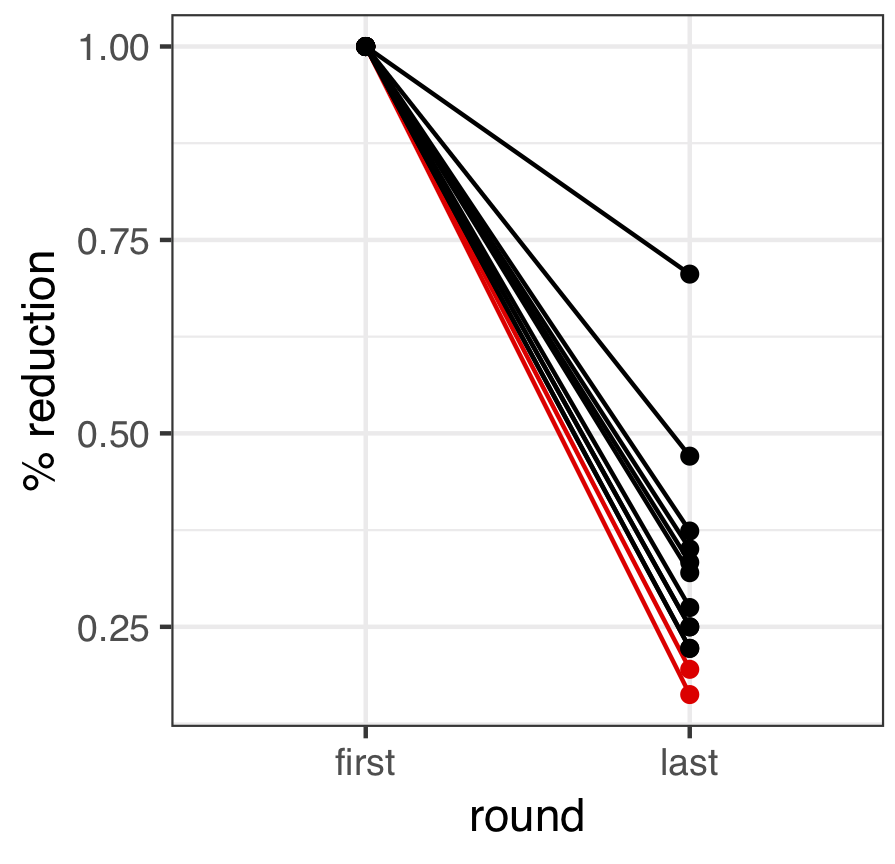
\includegraphics[scale=0.85]{reduction.png}
%\caption{Reduction in message length under different feedback conditions. Fifteen repeated reference game experiments are included: Krauss \& Weinheimer (1964) and Clark \& Wilkes-Gibbs (1986) are marked in red.}
%\label{fig:reduction}
%\end{figure}


Despite these underwhelming early results, the context-sensitivity of lexical priors remains a tantalizing area to revisit. Sources of variance in lexical expectations across speakers \cite{KingSumner15_VoiceSpecificSemantics}, and mechanisms supporting speaker-specific expectations \cite{TesinkEtAl09_MeaningfMRI,VanBerkum08_NeuralSpeakerMessage} may be more amenable to study using modern tools. In particular, more recently developed methods for measuring subjective beliefs and expectations \cite<e.g.>{FrankeEtAl16_CrowdBelieve, DelaneyBuschEtAl17_Cogsci} could provide much more direct access to underlying lexical beliefs, and large-scale online experiments could more systematically uncover the underlying structure of social group representations along which lexical expectations are organized. 

\section{Mechanism \#2: Rapid lexical learning}

If our lexical priors -- our global conventions -- serve as a source of stability in meaning over longer timescales, then what accounts for our extraordinary flexibility  over short timescales? How do we coordinate on efficient local conventions, or \emph{conceptual pacts}, for talking about things we've never talked about before? In this section, we review the dynamics of coordination within repeated reference games and explore the possibility that rapid adaptation can be understood in our hierarchical Bayesian modeling framework as lexical inference given partner-specific data: $P(\mathcal{L}_i | D_i, \Theta)$. 

\subsection{Convergence on efficient conventions}

The most well-known phenomenon in repeated reference games is a reduction in message length over multiple rounds. \citeA{KraussWeinheimer64_ReferencePhrases} were the first to report this phenomenon in a short technical report introducing the repeated reference game paradigm, and it has been replicated many times under many conditions \cite<most notably by>[in a much more streamlined experimental design using tangram shapes]{ClarkWilkesGibbs86_ReferringCollaborative}. Out of historical interest, it is worth describing the original design in detail. 

Both players were given an identical set of 6 cards marked randomly with 1-6 and A-F, respectively, containing the same 6 drawings in different orders. The pair's goal was to figure out the correspondences between their 6 cards by talking about the locations of the images. In each set, three images were `redundant,' appearing in the same location on every card---discussing these was not very useful for the task---while the other three were `diagnostic' and necessarily had to be referred to. This design therefore had the peculiar property that different drawings appear with different frequencies: some objects were referred to nearly 100 times (e.g. if diagnostic for every set of cards across all 16 rounds) and others only a handful of times. 

Their core descriptive result was that, taken in aggregate, frequently mentioned targets tend to be labeled using shorter phrases than infrequently mentioned targets, thus reproducing Zipf's law within the microcosm of a single conversation. To explain the process by which such a distribution emerges, they reasoned that labels may change with repeated use over the course of interaction. Indeed, the first time participants referred to a figure, they used a lengthy, detailed description (``the upside-down martini glass in a wire stand'') but with a small number of repetitions -- between 3 to 6 times, depending on the pair -- the description was reduced down to the limit of just one or two words (``martini''). 

%Rather than talking about slabs and bricks, as Wittgenstein's builders did, these participants were presented with an array of abstract line drawings. %This design was somewhat convoluted compared to later studies refining the paradigm but it's worth considering in detail, as it's the prototype from which all later studies derived.

% The most significant conceptual replication of this effect was conducted by . This streamlined version honed in on the process of social reasoning that allowed partners to successfully use short labels by the end. In their version of the task, participants were given boards containing the same 12 abstract tangrams (see Fig. 1b for a subset) but in scrambled orders. One participant -- the ``director'' -- was assigned to move sequentially through the grid, describing each one so that the other player -- the ``matcher'' -- can rearrange their tangrams to match. Critically, once the pair reached consensus and received feedback about mismatches, their tangrams are re-scrambled and they repeat the task for a total of 6 rounds. Thus, each of the 12 objects were referred to exactly 6 times. 

Note that although initial messages are just as long or longer than the other-intended messages collected by \citeA{FussellKrauss89_IntendedAudienceCommonGround}, final messages are as short or shorter than the one-shot messages intended for \emph{oneself}. Furthermore, final messages are often incomprehensible to overhearers who were not present for the initial messages \cite{SchoberClark89_Overhearers}. This observation sets up the central empirical puzzle of convention formation: how does a short word or phrase that would have been completely ineffective for communicating under the initial lexical prior become perfectly understandable over mere minutes of interaction? What changes inside participants' minds in the interim? 

One simple non-social explanation --- that reduction is merely an effect of familiarity or repetition on the part of the speaker --- can be easily dispelled. When participants are asked to repeatedly refer to the same targets for a hypothetical partner, no reduction is found, and in some cases utterances actually get longer \cite{HupetChantraine92_CollaborationOrRepitition}. Whatever is changing must be a result of the \emph{interaction} between partners. An alternative explanation suggested by our probabilistic model is that reduction is driven by lexical learning as communication partners coordinate on ad hoc names. If long initial messages can be explained as the result of initial uncertainty in the lexical prior, as discussed in the previous section, then a decrease in uncertainty licenses shorter messages \cite{HawkinsFrankGoodman17_ConventionFormation}. 

\subsection{Signatures of reduction}

What are empirical cues to this reduction in uncertainty? The first is the use of \emph{hedges}. Hedges are expressions like \emph{sort of} or \emph{like}, and morphemes like \emph{-ish}, that explicitly mark uncertainty or provisionality, such as \emph{a car, sort of silvery purple colored} \cite{BrennanClark96_ConceptualPactsConversation,Fraser10_Hedging,MedlockBriscoe07_HedgeClassification}. If participants reduce their lexical uncertainty over successive rounds, then we might expect a corresponding decrease in explicit markers of this uncertainty. \citeA{BrennanClark96_ConceptualPactsConversation} counted hedges over four repetitions of an initially ambiguous target and found widespread use of \emph{hedges} on the first round (occurring 26\% of messages) but almost complete absence on the last (only 2\% of messages). They also found very few initial hedges for targets with low initial uncertainty (e.g. a shoe in the context of dogs and fish), providing additional evidence for the role of \emph{lexical} uncertainty as opposed to a generic social use of hedges.

Another characteristic of uncertainty reduction lies in \emph{what} gets reduced, which we discuss in depth in Chapter 4. 
Is the speaker adopting a fragment shorthand by randomly dropping function words, or are they simplifying or narrowing their descriptions to names by omitting redundant details? Closed-class parts of speech like determiners and prepositions \emph{are} much more likely to be dropped than open-class parts of speech like adjectives and nouns. But when we examine broader grammatical units using recent NLP techniques, we find that entire modifying clauses are increasingly likely to be dropped \cite{HawkinsFrankGoodman17_ConventionFormation}. This accords with early hand-tagged analyses by \citeA{Carroll80_NamingHedges}, which found that in three-quarters of transcripts from \citeA{KraussWeinheimer64_ReferencePhrases} the short names that participants converged upon were prominent in some syntactic construction at the beginning, often as a head noun that was initially modified or qualified by other information. 

%\todo[inline]{Mention shift from indefinite to definite? Clark \& Wilkes-Gibbs (1986)}

These more fine-grained analyses suggest that reduction is grounded in the prior lexical content of the interaction and the speaker's increasing confidence in how the listener will interpret an initially ambiguous label. Like the evidence we reviewed about lexical priors, however, this evidence remains indirect and raises the need for more careful, direct measurement of lexical uncertainty over interaction. 

\subsection{Quality of feedback}

If adaptation is learning, then the extent to which partners adapt should depend critically on the quality of the data $D_i$ on which they are conditioning: $P(\mathcal{L}_i | \Theta, D_i)$. In the absence of additional cues to the meanings that their partner is using to interpret their messages, a speaker or drawer can only continue to rely on their prior, or indeed elaborate upon it. A common feature of the reference games reviewed so far is the capacity for \emph{real-time feedback channel}: either player may say anything at any point in time, thus allowing for interruptions, back-channel responses (uh-huh, hmmm, huh?), clarification questions, and so on. To what extent is this design choice necessary for reduction? \citeA{KraussWeinheimer66_Tangrams} were the earliest to address this question by manipulating the kind of feedback received by the speaker.

% In one condition, participants were able to talk freely and bidirectionally as in \citeA{KraussWeinheimer64_ReferencePhrases}; in another condition, the channel was unidirectional: the speaker was unable to hear the listener's responses. This real-time feedback manipulation was crossed with a behavioral feedback manipulation where the experimenters intercepted the listener's responses: one group of speakers was told that their partner made the correct response 100\% of the trials (regardless of their real responses), while another was told on half of the trials that their partner made the incorrect response. 

Intuitively, we might expect that if the speaker is unsure how their longer descriptions are being interpreted -- unsure whether or not they can get away with shorter, more ambiguous expressions -- they may not have enough evidence about meanings to justify shorter utterances. Indeed, \citeA{KraussWeinheimer66_Tangrams} found that even when told that their partner was getting 100\% correct, entirely blocking the verbal feedback channel significantly limited the reduction effect. Speakers converged to utterances that were about twice as long -- twice as inefficient -- in the limit. Telling speakers that their partner was performing poorly also inhibited reduction as a main effect, though to a lesser extent. In the extreme case of trying to communicate to a listener who can't respond and appears to not understand, speaker utterance length actually increased with repetition after an early dip. \citeA{HupetChantraine92_CollaborationOrRepitition} later found that in the \emph{complete} absence of feedback --- when the speaker is instructed to repeatedly refer to a set of objects for a listener who is not present and will do their half of the task offline --- there is also no reduction in message length. On the listener's part, too, the ability to actively \emph{give} feedback appears critical for learning. \citeA{SchoberClark89_Overhearers} showed that listeners who overheard the entire game were significantly less accurate than listeners who could directly interact with the speaker, even though they heard the exact same utterances.

More graded disruptions of feedback seem to force the speaker to use more words overall but not to significantly change the rate of reduction (though rigorous comparisons between rates have not been conducted). For example, \citeA{KraussBricker67_Delay} tested a transmission delay to temporally shift feedback and an access delay to block the onset of listener feedback until the speaker is finished. Later, \citeA{KraussEtAl77_AudioVisualBackChannel} replicated the adverse effect of delay but showed that undelayed visual access to one's partner cancelled out the effect and returned the number of words used to baseline. 

%\todo[inline]{Mention that negative feedback can be useful too -- cf Horton \& Gerrig, 2002 arguing that speakers `learn that audience design is necessary' and intentionally try to counteract the tendency to shorten by lengthening more for the second partner.}

\subsection{Why so fast?}

Some access to minimal feedback from one's partner therefore appears to be a necessary condition for convention formation. Without it, there is no reliable cue to the partner's lexicon; no lexical learning can take place, and consequently no social coordination. Yet this condition alone doesn't explain the \emph{speed} with which partners adapt, approaching `one-shot' learning. Three additional factors seem relevant. 

First, like other scenarios of rapid learning from sparse data, abstract prior knowledge is crucial \cite{TenenbaumKempGriffithsGoodman11_Grow_a_Mind_Science,LakeEtAl16_BuildingMachines}: agents do not start from scratch, they must only fine-tune their pre-existing global conventions to fit their immediate partner and context. Second, agents have pragmatics on their side. In the RSA model linking lexical knowledge to behavior, listeners assume their partner is attempting to be \emph{informative} and pragmatic speakers, in turn, \emph{expect} listeners to do so. These assumptions dramatically strengthen feedback. Because listeners reason about alternatives -- that the speaker \emph{would} have used another word or description if it described the target better in context -- both agents actually learn about the meanings of words that were not uttered\footnote{
This is the \emph{lateral-inhibition} dynamic described at length by \citeA{Steels03_GroundedCommunication,SteelsEtAl05_CoordinatingColors,Steels15_TalkingHeadsExperiment}, which emerges naturally in our model from basic Gricean principles.
}. Similarly, the existence of a listener backchannel (knowing a listener \emph{would} object or ask for clarification if their lexicon differed) implies evidence for the utterance's meaning in the absence of such objections. A third factor is the sociolinguistic information derived from social group inferences, which are often tightly controlled in lab settings but likely more relevant in the real world. 

\subsection{Social group inference}

In addition to updating our model of a particular partner based on immediate feedback, i.e. utterances and choices made in previous rounds of the game, a hierarchical Bayesian learning model predicts that sparse observations of a partner's language use may license much broader inferences about their lexicon via diagnostic information about their social group or background. If someone's favorite song is an obscure B-side from an obscure punk single, you can make fairly strong inferences about what else they like to listen to and how similar they might be to you \cite{VelezEtAl16_Overlaps, GershmanEtAl17_StructureSocialInfluence}. Similarly, if someone casually refers to an obscure New York landmark you also recognize, you can safely update your beliefs about their lexicon to include a number of other conventions shared among New Yorkers. Lexica cluster within social groups, so inverting this relationship can yield rapid lexical learning from inferences about social group membership.

This source of lexical learning was explored in a study by \citeA{IsaacsClark87_ReferencesExpertsNovices} where novices and experts were paired for a repeated reference game using postcards of New York landmarks. Both directors and matchers could be either novices or experts, creating a 2x2 design. While a strong main effect of reduction was found across all pairings of experts and novices, they differed strikingly in their use of proper nouns (i.e. conventions shared by experts). For instance, over the course of the experiment, experts consistently used short messages with proper nouns (e.g. ``the Rockefeller Center'') when talking to other experts, while novice directors gradually adapted to expert matchers, doubling their use of proper names (and therefore drastically reducing the length of their utterances).

Most striking, however, was the observation that directors had already adapted in the first few trials of the first round: by the fourth round expert directors were already using a proper noun three times more often when talking to other directors than in talking to novices. In fact, independent raters were presented with transcripts from the first two postcards and correctly judged the expertise of the two partners 84\% of the time. This is a straightforward prediction of a hierarchical Bayesian model: given a latent group representation of New Yorkers, a director can make a strong prediction that if their partner belongs to this group, ``Rockefeller Center'' will belong to their lexicon with high probability. Hence, any interpretation failure is strong evidence that their partner is not in the group and is thus equally unlikely to recognize ``Citicorp Building'' or ``Brooklyn Bridge''. In this way, convention formation and social group inference are intimately intertwined. 

\section{Mechanism \#3: Generalization}

If the local conventions -- or pacts -- formed over the course of an interaction reflect learning, then what are the boundaries of that learning? How does meaning in one context with one partner transfer to expectations about new contexts and new partners? %When can a peculiar meaning be explained away as the idiosyncrasy of a particular partner, and when does it become a generic lexical expectation or global convention?
In this section, we discuss three empirical properties of generalization that computational models of convention formation must account for. Over short time scales, lexical pacts are \emph{partner-specific} but stable across \emph{contexts}. 
Over longer time scales, however, as agents repeatedly interact with multiple partners in larger social networks, pairwise conventions generalize to global conventions expected to be shared across the entire \emph{community}.
A mechanism for generalization, then, is not only key to understanding the appropriate scope of local conventions, but also where our global conventions came from in the first place.

\subsection{Partner-specificity}

One of the most salient and well-studied properties of local conventions is precisely that they \emph{don't} generalize immediately to novel partners. In other words, the speaker is learning a specific model of their partner on the basis of shared history, not just privately forming an association between words and objects. This can be demonstrated in a repeated reference game by  swapping in a novel parter after several rounds of interaction (\citeNP{WilkesGibbsClark92_CoordinatingBeliefs}; see also \citeNP{BrennanClark96_ConceptualPactsConversation}, \citeNP{WeberCamerer03_CulturalConflict}, \citeNP{YoonBrownSchmidt14_ConceptualPacts} for variations on this design). If the speaker's lexical representation did not distinguish between partners with different histories, then we should expect no difference before and after this intervention. Instead, \citeA{WilkesGibbsClark92_CoordinatingBeliefs} found that speakers immediately reverted to longer messages---a 275\% increase---bringing them nearly back to the length of the initial messages used with the original partner. 

Other interventions explore intermediate cases, where the swapped-in listener was not \emph{entirely} novel. For example, when \citeA{WilkesGibbsClark92_CoordinatingBeliefs} introduced them as a ``silent participant'' during the first phase, sitting at the same table as the speaker and able to make eye contact, there was only a 67\% increase in message length. When they were an \emph{omniscient bystander}, observing the audio and visuals of the entire exchange from a separate room, length increased slightly more (100\%). Finally, when they were a \emph{simple bystander}, seated some distance behind the director such that they could not be monitored or see the tangrams being referred to, length increased as much as with a fully novel partner. 

These graded effects reflect degrees of \emph{partial information} about the swapped-in listener's beliefs, posing a challenge even for computational models that allow partner-specific learning. It is simple for a hierarchical learning account to explain why speakers had no particular expectations about the \emph{simple bystander}, who could not see the tangrams that were being referred to and therefore was not provided with the relevant data to learn meanings. But for third parties who \emph{did} have full access to the interaction, whatever additional information the speaker is using cannot be limited to the assumption that the swapped-in listener can consult the same data, otherwise the \emph{omniscient bystander} should be treated the same as the \emph{silent participant}. 

One explanation, which could plausibly be incorporated into a learning model, is that although the silent participant cannot verbally respond, they do nonetheless provide a minimal feedback channel through their physical presence, e.g. eye contact or body language. Because they are co-present at the table, they belong to the intended audience for the speaker's messages, and can be monitored for cues to understanding; this evidence in turn may not indicate partner generalization per se, but joint learning about the two listeners. 

A related question concerns how partner identity is cued or inferred: even for a model that learns partner-specific lexical representations, the identity of a particular partner may be noisy, requiring inference under uncertainty about what is in common ground. In a challenging task used by \citeA{HortonGerrig02_AudienceDesign}, a speaker played several rounds of a repeated reference game with two listeners at once. Critically, each listener only had access to a \emph{subset} of the total grid of targets in front of the speaker, which the speaker could only learn through interaction. Having converged on local conventions for one set of objects with listener A and for another set of objects with listener B, the speaker was then put in a test phase where they had to communicate \emph{all} objects with each listener separately. %Again, if their representation didn't take into account partner-specific histories of interaction, they should treat all objects as equally shared for both partners. 
As a main effect, \citeA{HortonGerrig02_AudienceDesign} found a small boost in message length for the subset of objects that \emph{weren't} originally part of the present listener's array, indicating that the speaker flexibly shifted their messages to accommodate the differing history with each listener. There was also evidence from intra-utterance analyses that partner-specific representations were used to form the very first messages and the effects weren't simply driven by low-level feedback (e.g. if the speaker began by producing the reduced label used with the previous partner, and only added additional information after the listener indicated trouble understanding). 

This result by itself is a small but compelling addition to the cumulative evidence of partner-specificity, but also presents two additional challenges for computational models related to the noisiness of partner-specific learning. First, there was a strong order effect, with a much stronger increase in message length at the \emph{second} test session (with partner B), suggesting some additional learning of what was in common ground with partner B in the first test session with partner A. Second, in a follow-up study, \citeA{HortonGerrig05_MemoryAudienceDesign} found that clustering the stimuli to facilitate easier learning of which objects were known by which speakers during the first phase significantly strengthened the partner-specific effect. These observations indicate that under challenging conditions, learning partner-specific representations is a noisy affair and often appears far from `optimal' even in a rational learning model. 

%A critical claim of our hierarchical model is that partner-specificity is an inherent property of the \emph{representations} used by the speaker, yet it is unclear from summary measures like average message length whether flexible adaptation to new partners is driven by partner-specific lexical expectations or simpler reactions to real-time feedback from the novel listener. For instance, . This latter mechanism is certainly at play \cite[see]{SchoberBrennan03_RoleOfThePartner}, but there does exist some evidence that partner-specific representations are used by the speaker even before receiving any feedback. 

Finally, while most repeated reference games have focused on testing speaker adaptation, there is evidence that partner-specific information is represented by the listener, too. For example, \citeA{MetzingBrennan03_PartnerSpecificPacts} tested the partner-specificity of listener representations in an eye-tracking study with a confederate \emph{speaker}. In one condition, after several rounds of interaction ``converging'' on a pre-scripted convention (e.g. \emph{``the shiny cylinder''}), the speaker \emph{broke} the pact, suddenly introducing a novel but synonymous term (e.g. \emph{``the silver pipe''}). In another condition, the speaker was replaced such that the novel term was produced by a novel speaker. In this latter case, the listener looked at the target just as quickly as when the old speaker produced the conventionalized term. However, when the \emph{old} speaker produced a new term, they found a significant delay in the listener's first look to the target. Listeners in this condition tended to gaze around the display for other objects, suggesting a momentary contrastive implicature. Because the only difference between the two utterances was the identity of the speaker, this provides good reason to believe that listeners also form partner-specific lexical representations over interaction. %This is consistent with our Rational Speech Act model under partner-specific lexical learning: if the speaker had intended the particular object which is best described by \emph{``the shiny cylinder''} in their partner's lexicon (as the listener has learned from usage in previous rounds), then they would have  

\subsection{Path-dependence and stability across contexts}

Another key computational signature of local conventions is their stability, or \emph{stickiness}, across changing contexts. Once a precedent has been established with a particular partner, the pressure to maintain it apparently even trumps the usual Gricean pressures of informativity in context. For example, suppose a pair of participants have converged on an sufficiently specific subordinate term like \emph{pennyloafer} after several rounds referring to a particular shoe in the context of other shoes. %Rather than swapping out the partner like the studies in the previous section, the experimenter can swap out the context, 
When subsequently placed in a new context where all but the target shoe have been replaced with objects from other categories, participants remarkably continued to use the now-overinformative label (e.g. \emph{pennyloafer}) 52\% of the time, even though it is the only shoe \cite{BrennanClark96_ConceptualPactsConversation}.

This can be understood in our model as a consequence of the path-dependence of lexical learning. The initial context affects the initial terms produced via the Gricean reasoning formalized in RSA. Using the basic-level label \emph{shoe} in the initial round would be under-informative because it applies to the distractor shoes equally well \cite{GrafEtAl16_BasicLevel}, but there are several appropriately informative alternatives under the lexical prior with approximately the same cost of production (\emph{pennyloafer}, \emph{docksider}, \emph{brown shoe}, \emph{dress shoe}). Which of these roughly equivalent labels the speaker samples, then, is somewhat \emph{arbitrary}: \citeA{BrennanClark96_ConceptualPactsConversation} found considerable variance in labeling with only a 10\% chance of matching labels across speakers (see also \citeNP{FurnasEtAl87_VocabularyProblem,HupetEtAl91_CodabilityReference}). 

After a successful round of reference with a particular one of these labels, however, lexica in which this label applies strongly to this particular shoe become more likely, and alternative lexica in which other terms apply better to that same shoe become less likely (by the same Gricean reasoning as earlier: if there were a better term in the partner's lexicon, they would've used it). This dynamic alone accounts for the stability and path-dependence of reference \emph{within} contexts \cite{HawkinsFrankGoodman17_ConventionFormation}. Empirically, \citeA{BrennanClark96_ConceptualPactsConversation} report significantly greater variability of labels across pairs than within pairs (see also \citeNP{HawkinsFrankGoodman17_ConventionFormation} for an information theoretic analysis of arbitrariness and stability on a larger data set). 

Extending this argument, it also becomes clear why path-dependent learning would stick across new contexts.  After several rounds of initial reinforcement, the evidence for the lexical meaning of a subordinate-level term (\emph{pennyloafer}) is so strong that when the context changes, the informativity of this term under the learned lexicon is strong enough relative to the prior uncertainty on the basic-level term (\emph{shoe}) to justify the small additional utterance cost. Critically, this same mechanism also predicts why conventions should \emph{not} generalize when the context switch goes in the opposite direction: when the initial context only contains one shoe, 89\% of speakers switched to a more specific utterance when additional shoes are added to the context \cite{BrennanClark96_ConceptualPactsConversation}. However much speakers strengthened their belief that \emph{shoe} refers to a particular shoe in the first context, it doesn't change the lexical prior of that term \emph{also} applying to the other shoes in the new context. Just saying \emph{shoe} would be extremely underinformative even under the learned lexicon, necessitating a more specific label.

Our lexical learning account also accounts for two additional phenomena related to stability reported by \citeA{BrennanClark96_ConceptualPactsConversation}: frequency and role independence. First, the more a local convention was initially reinforced, the stickier it was: participants were half as likely to switch to \emph{shoe} from the more specific \emph{pennyloafer} when they did 4 repetitions of \emph{pennyloafer} in the specific context than when they only did 1 repetition. Second, in an experiment when the pair switched roles at the same time as the new context is introduced, this pattern of results stayed the same, indicating that coordinated lexical learning is taking place for both partners. 

The stickiness of conventions has been challenged recently by \citeA{MisyakEtAl16_InstantaneousConventions} using a repeated reference game where the communication medium was placing tokens instead of words. They showed that depending on contextual and environmental constraints, the same `message' (placing a token on a box) can flip its meaning from trial-to-trial in completely contradictory ways. The one-shot pragmatic reasoning allowing for this degree of semantic flexibility presents a fascinating case for lexical uncertainty RSA models, but we strongly disagree that what is being described is a \emph{convention} in any sense discussed in this article via the tradition of \citeA{Lewis69_Convention}. The severe simplicity of their synchronic scenario (binary signals and binary referents constructed such that there is a single `optimal' best-response strategy on any trial regardless of prior beliefs) obviates any functional need for diachronic learned representations or dependence on common ground across trials. In particular, a defining property of conventions in is their \emph{arbitrariness}: there needs to exist an alternative that \emph{would} be equally successful if everyone agreed (e.g. participants who use \emph{docksider} are just as successful as those who use  \emph{pennyloafer}). There is no such arbitrariness in \citeA{MisyakEtAl16_InstantaneousConventions}, as indicated in their own data showing almost no variability in what participants do on a given trial type. If even the most minimal arbitrariness were introduced, for example two colors of tokens, we predict the usual sticky conventions would form: some participants would begin to persistently associate a particular meaning with `blue' and others would associate it with `yellow.' %While \citeA{MisyakEtAl16_InstantaneousConventions} pose an interesting phenomenon for models of one-shot pragmatic reasoning to account for, then, we don't see any bearing on general models of convention formation.

%\subsection{Generalization from object to categories}
%
%\cite{MarkmanMakin98_ReferentialCommunicationCategory}
%
%\cite{MaltSloman04_ConversationConvention}

\subsection{Generalization from local to global conventions}

The first two sections of this paper focused on how global conventions -- our lexical priors -- shape the formation of local conventions. 
They seed the initial expectations we bring into interactions, getting communication off the ground and scaffolding rapid lexical learning. %All the repeated reference games we've reviewed %in the tradition of Krauss \& Weinheimer (1964) and Clark \& Wilkes-Gibbs (1986) 
%implicitly rely on the fact that participants share the same native tongue to get communication off the ground. For instance, the lengthy initial descriptions key to reduction are only useful because the speaker has relatively strong priors about the meanings of words in general, even if those global conventions aren't sufficient for efficiently naming these particular novel stimuli in this context. 
But what about influence in the other direction? 
Where do global conventions come from in the first place? Some are certainly \emph{iconic} and based on expectations about resemblance in shared perceptual systems \cite{DingemanseEtAl15_IconicityLanguage,VerhoefKirbyBoer16_Iconicity}.%,DingemanseEtAl16_SoundSymbolism}. 
Yet for the essentially arbitrary form-meaning mappings that make up the bulk of our lexicon, it is difficult to imagine any mechanism for their emergence that doesn't first pass through local conventions. How do interactions with one partner shape the prior one brings into interactions with other partners, and how do these priors converge across social networks? 

\begin{figure}[t]
\centering
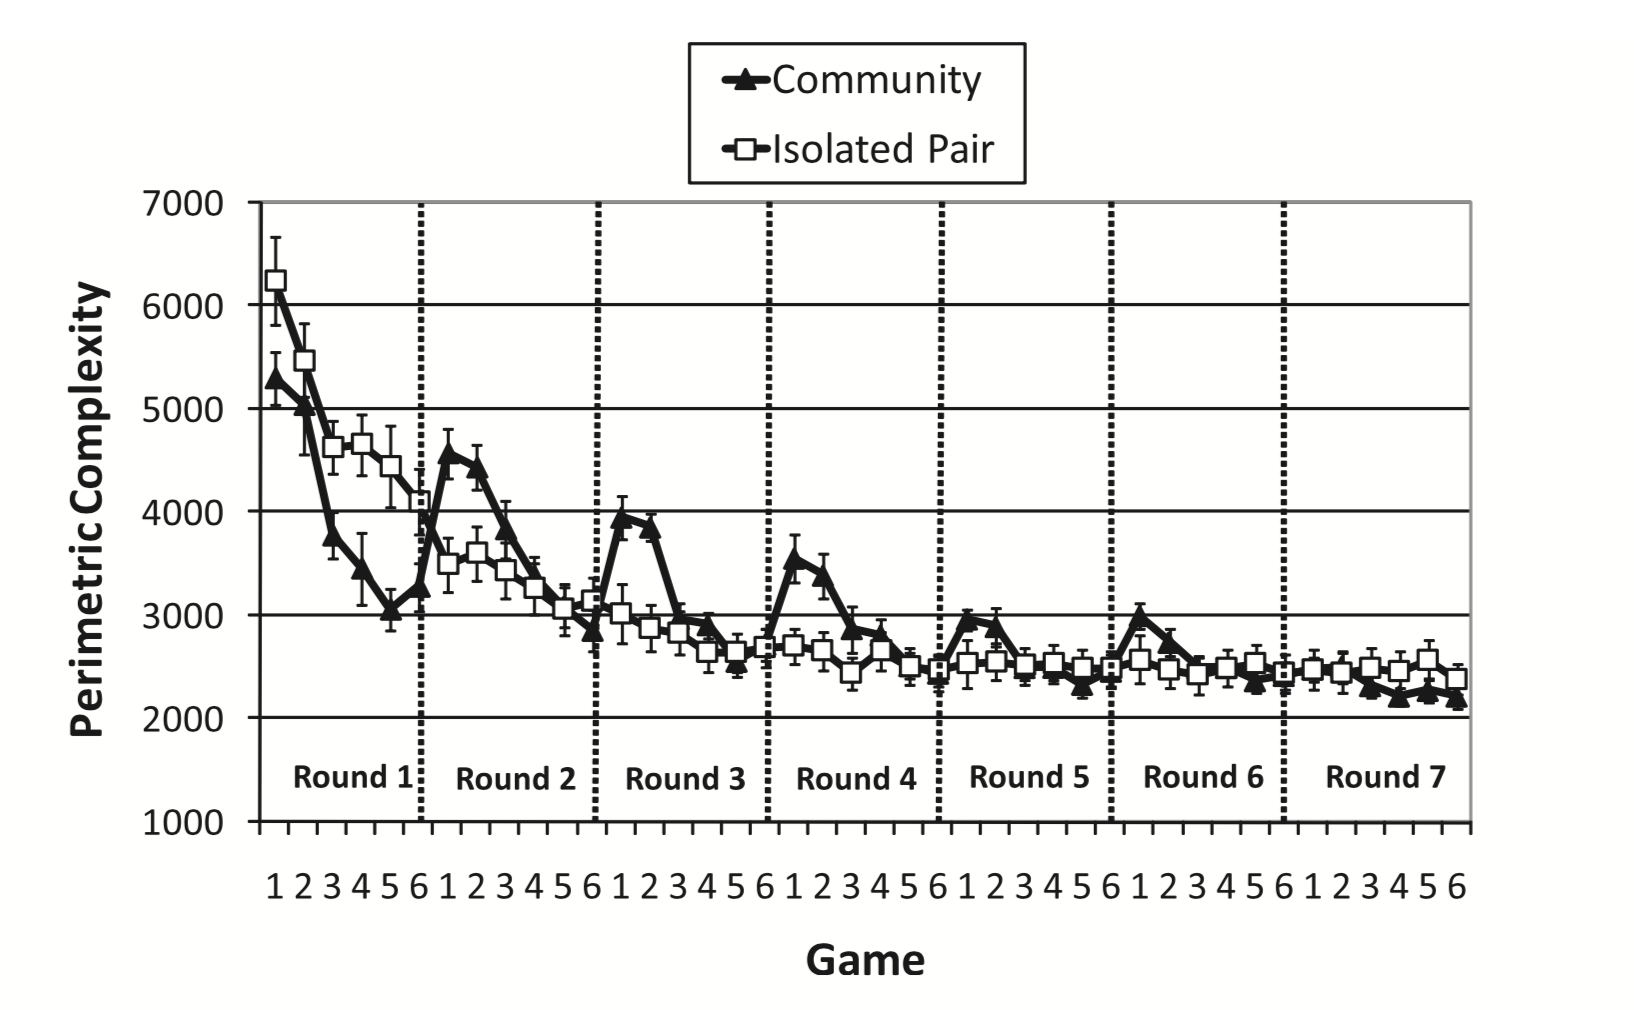
\includegraphics[scale=0.5]{FayEtAl10_Results}
\caption{Reduction and conventionalization across a community, compared to a single pair. At each vertical line, participants in the ``Community'' condition switched partners; at each switch, the complexity of their drawings increases, but by less and less as they converge on a shared set of global expectations as efficient as the isolated pair formed over an equal number of games. Reproduced from Fay et al. (2010).}
\label{fig:community}
\end{figure}

%Although repeated reference games have not been systematically conducted with larger groups, several points of evidence are relevant. 
One simple prediction of our hierarchical learning model is that repeated pairwise interaction within a particular community should lead to convergence within the community as participants begin to generalize across partners. \citeA{FayGarrodRobertsSwoboda10_InteractiveEvolution} tested this prediction by dividing participants into several `communities' where they played several rounds of a \emph{graphical} repeated reference game with each member of their community (see below for more discussion of modality differences). Although early partner swaps led to sharp losses in efficiency---consistent with the partner-specificity of conventions---these losses gradually disappeared over successive swaps (see Fig. \ref{fig:community}), indicating eventual community-level convergence on expectations as strong as those found in isolated pairs \cite<see>[for similar results in a more complex communication game]{GarrodDoherty94_GroupConventionsLinguistics}. 

A corollary of this in-group convergence is that communication should be \emph{hindered} when assumptions about global priors are violated. When a similar within-group convergence phase was followed by a `test' phase where participants are either paired with a novel member of their own community or a member of a \emph{different} community (without being explicitly told which it is), sketchers in the latter condition required significantly more ink to succeed. %In this game, they concurrently drew sketches on the same sketchpad to determine whether pieces of music they heard were the same or different, and no target pieces were repeated. 
%Thus, players are increasingly likely to be paired with others who have an indirect connection in the network---who have also met their previous partners or partner's partners. 
Because no target was referred to more than once with the same partner, whatever alignment of expectations took place over the course of in-group training had to be generalized \emph{across} partners via the overall prior. Note that the network topology implicitly used in these studies (homogenous mixing on a complete graph) is likely critical to this convergence: \citeA{CentolaBaronchelli15_ConventionEmergence} found that  simpler coordination games embedded on other common topologies---low-degree lattices and random graphs---tend to get stuck with local regions of the network using incommensurate conventions. 

Over longer (generational) time scales, the emergence and stability of community-wide conventions plays a functional role in cultural and linguistic continuity. The composition of a community is constantly shifting as old members die and new members are born: without a mechanism for partner-specific learning to transfer into global beliefs, communication systems would have to be reinvented at each generation. These intergenerational mechanisms have been investigated in the laboratory using replacement or micro-society designs.%\cite{GerardKluckhohnRapoport56_Replacement}. 
For instance, \citeA{CaldwellSmith12_Conventions} conducted a reference game where a speaker tried to get three listeners to guess color terms by drawing on a sheet of paper. After referring to each color only once, they were replaced by the most senior listener, and a new listener was cycled into the audience. After several rounds, the group was completely different from the original, yet patterns of reduction and path-dependent conventionalization were broadly the same as when a single pair plays repeatedly. 

Granted, this particular result could be adequately explained by a non-hierarchical but partner-specific learning model. Because the speaker only had to get \emph{one} of the listeners to guess correctly, they could have relied on the partner-specific models built up for two of their three audience members on previous rounds while simply ignoring the novel partner. But in more extreme cases of pair-wise interactions with population turn-over, we nonetheless predict that global conventions would emerge and persist across generations.\footnote{
Note that actual communication within the lifetime seems crucial for this process: pure iterated learning does not produce conventionalization \cite{GarrodEtAl10_IteratedLearningGraphicalSymbols})
}

%each player engages in one-shot interactions with multiple partners. These games nonetheless present a special case for hierarchical learning models, where there is no opportunity for partner-specific learning and speakers must assume all partners are drawn from the same population. In one large-scale web experiment, participants were placed on one of three social networks with different topologies \citeA{CentolaBaronchelli15_ConventionEmergence} On each round, each player was randomly paired with one of their neighbors on the network and simultaneously typed names for a displayed human face that was the only referent in the whole game. They were rewarded if the names exactly matched and penalized otherwise. Whether or not the whole population converged on a shared global convention depended strongly on the topology: certain topologies had a risk of  homogenously mixing topologies, local clusters converged internally but

\subsection{Generalization in language acquisition}

Finally, there is a particularly fascinating developmental parallel raised by these hierarchical learning mechanisms. Are the lexical learning mechanisms adults use to coordinate on local conventions \emph{within} an interaction the same as those supporting language-learning more broadly? Most laboratory tasks investigating cross-situational word learning only use a single speaker, and even sophisticated models of cross-situational word learning that account for pragmatic reasoning about speaker intentions \cite[e.g.]{FrankGoodmanTenenbaum09_Wurwur} tend to collapse over \emph{who} is talking. Yet, as we have argued throughout this article, there is substantial variability across different speakers. If the majority of child-directed speech only comes from a single primary caregiver, then the child may face a difficult generalization problem once they begin interacting with others. Upon hearing an unfamiliar word from a novel speaker, or a familiar word utterance with an unfamiliar meaning, it could be a quirk of that particular speaker \emph{or} indicative of a globally shared convention. There may therefore be substantial path-dependence in acquisition, as children develop their lexical prior and become better attuned to the overall variability in the population \cite<see>[Chap. 6]{Clark09_FirstLanguageAcquisition}. 

This slow-developing lexical prior is one of several explanation for why young children are so terrible at coordinating on local conventions in repeated reference games \cite{GlucksbergKraussWeisberg66_DevoRefGames,KraussGlucksberg77_SocialNonsocialSpeech}. When an experimenter feeds them the messages that adult speakers produced naturally, they had no trouble, even as they reduced down to one- or two-word utterances. When they played with one another, however, Kindergardeners continued to make errors even after 15-16 repetitions; children as old as fifth grade only improved with assistance from the experimenter and never approached the perfect levels of adult performance. Instead of beginning with the long indefinite descriptions full of hedges and modifiers that adults provide, nursery-school speakers began with short, highly idiosyncratic descriptions like \emph{Mother's dress}. If adult speakers' long hedge-filled messages are indeed motivated by lexical uncertainty, then perhaps young children have simply not obtained enough linguistic variability to calibrate their lexical prior. Alternatively, if the pragmatic reasoning required to produce informative utterance depends on theory of mind, then the high processing demands of the task may simply be inhibited performance \cite<e.g.>{SetohScottBaillargeon16_FalseBelief}. This remains an underexplored puzzle for future developmental research. 

\section{Discussion}

Repeated reference games provide a rich arena for studying social interaction and adaptation. Initial utterances expose the global conventions people bring into novel interactions, and how people incorporate contextual information into their expectations. Successive rounds demonstrate the remarkable speed and flexibility with which people form local conventions to successfully coordinate their behavior. Finally, by intervening in these games to manipulate partner or context, we can reveal the boundaries of learning through tests of generalization. 

Throughout, we have argued for a probabilistic model where agents initially have uncertainty over the latent representation guiding their partner's actions and dynamically coordinate over time by conditioning on shared history. 
A critical component of this model is the hierarchical structure by which all members of a community are assumed to be drawn from a distribution with shared parameters, allowing a pathway for global conventions to be influenced by local interactions without sacrificing the ability to learn idiosyncratic partner-specific models. 
This account situates convention formation as the product of generic hierarchical learning machinery operating on social data.

Although our brief sketch of this model provided a useful conceptual framework for synthesizing diverse convention formation phenomena, there remain many computational details to work out before it could be effectively deployed, for example, as an AI capable of coordinating with humans in real-time. 
The scope of this review was limited to the broad behavioral phenomena uncovered by repeated reference games, but going forward, it will also be important to (1) tie this computational-level account to underlying neural and algorithmic mechanisms for adaptation and (2) contrast our learning account with both simpler low-level `priming' based models and richer collaborative notions requiring recursive `mutual knowledge.' Before closing, we briefly touch on two broader discussion points: the domain-generality of convention formation across multiple modalities and the additional levels of coordination for which learning must take place.

\subsection{Coordination at other levels}

While we have thus far limited our discussed specifically to the reduction and simplification of messages as participants coordinate on meanings given a shared set of referents, this is only one of many levels at which conventions can form. In more complex circumstances, there is often initial uncertainty not just about which of a small set of targets a particular message refers to, but how to represent the relevant targets of reference in the first place. For instance, when using sketches to communicate about the identity of complex pieces of music \cite{HealeySwobodaUmataKing07_GraphicalLanguageGames}, a particular set of strokes could correspond to any number of properties (pitch, tempo, melody, rhythm, intensity) at any temporal granularity. This is made particularly clear in the classic maze game \cite{GarrodAnderson87_SayingWhatYouMean}: in order to give effective spatial directions, speakers had well-tuned lexical priors but had to coordinate on what space of \emph{referents} to use (e.g. paths, coordinates, lines, landmarks). Our probabilistic model can be extended to handle additional levels of coordination by placing uncertainty over a hyperparameter corresponding to the intended feature dimension that must be jointly with the corresondance along that dimension. 

Throughout this paper, we assumed that stimuli like tangrams were fixed objects in fixed categories and all learning happened over the mapping from words to these objects or categories. The present discussion, however, raises the possibility that people are not in fact coordinating on \emph{lexical meanings}, but pushing the uncertainty back a level and coordinating instead on how to categorize the object. Perhaps meanings are fixed and the only learning taking place is how one's partner construes a multi-stable percept. This seems to be what \citeA{BrennanClark96_ConceptualPactsConversation} had in mind when they coined the term \emph{conceptual pact}. Given present data it is not clear how these two sources of uncertainty could be teased apart, though certain conventions (e.g. proper names or acronyms) are clearly not issues of conceptualization; both levels of coordination are likely to play a role. 

%\todo[inline]{Garrod \& Anderson, 1987 Mazes}
%\todo[inline]{Schober, 1993?
%``When interlocutors face each other, terms like on the left are ambiguous depending on whether the speaker takes what we can call an egocentric or an allocentric reference frame. Schober found that if, for instance, A said on the left meaning on A's left (i.e., an egocentric reference frame), then B would subsequently describe similar locations as on the right (also taking an egocentric frame of reference)''}
%\todo[inline]{Dale et al, 2011: Don't analyze linguistic data but show that eyes/hands become coordinated over course of tangrams task}

%Nonetheless, Galantucci found that most partners were able to jointly learn a shared communication system to solve repeated spatial coordination tasks in a relatively short span of time. In the simplest version of this task, each player was placed in one of four rooms on a map, with the identity of a room marked only by large symbols. They were rewarded for finding one another in one room-change or less, and therefore needed to use their communication channel to convey information about their position and where to go. Note that this game contains the same basic structure as a basic tangram-style reference game where there are four `targets' (rooms marked by shapes) that must repeatedly be referred to: it is just embedded inside a considerably more complex set of strategic and spatial challenges. The average time to converge on an effective system was a little over an hour. 
%
%From the perspective of learning, this is an incredible feat: because participants were basically told nothing before beginning play, they had to infer the spatial structure of the map, the categorical structure of strokes used by their partner (e.g. when are two distinct percepts the same `sign'), the meaning of each stroke (e.g. which stroke corresponds to which room? Is it a request like `let's go here' or a statement like `I am here'?), and so on, all from fairly sparse and noisy feedback. Unfortunately, any universal conclusion about how participants managed this feat was difficult to draw: only ten pairs played the game, and essentially every pair found a different solution. Still, these solutions bear the same qualitative signatures of the convention formation process found in all iterated communication games: when prior conventions are not sufficient for the task at hand, partners rapidly learn arbitrary and path-dependent but stable solutions from observing one another's behavior in early rounds. 

%\todo[inline]{brief call-out to, like, Selten \& Warglien, 2007 where dyads used ``string of permissable letters'' like ``RM''? Not quite reference game b/c both players typed messages that had to match? Main focus was on compositional grammar? }
%
%\subsection{Underlying mechanisms}
%
%Partner-specific representations, N400? \cite{TesinkEtAl09_MeaningfMRI,VanBerkum08_NeuralSpeakerMessage}
%
%Declarative memory (hippocampus?) \cite{DuffBrownSchmidt12_Hippocampus}
%
%Time-course questions? \cite{HortonGerrig16_MemoryBasedReview}

%\subsection{Other theories and models of convention formation in repeated reference games.}
%
%Our assumption of a probabilistic, context-sensitive lexical prior can be contrasted with the more dominant view of the lexicon as a monolithic representation of lexical knowledge acquired across our individual experience with language use. Instead of engaging theory of mind to represent a partner's lexicon, then, we could just heuristically substitute our own representation as an approximation   \cite{Steels03_GroundedCommunication,JonesEtAl15_SemanticMemory}. %This position is typical of process-level models focusing on, 
%Note that this `egocentric' heuristic would be completely rational under strong conventional assumptions of common ground: if everyone assumes mutual knowledge of this lexicon is shared across their community, then it is in everyone's best interest to adhere to identical meanings, and reasonable to expect that a particular partner in the community is doing so. Yet we will see that it falls short in accounting for partner-specific effects.
%
%A number of distinct theoretical accounts have been offered to make sense of pieces of this large body of results. These accounts roughly divide into two camps: the `minimalists' and the `maximalists.' The minimalists seek to identify the simplest set of mechanisms that, when implemented in a communicative agent, will give rise to some conventional phenomena. Often these mechanisms involve low-level priming or simple `if-then' heuristics and strongly reject the need for any representation of `other-modeling.' The maximalists, on the other hand, argue that partner-specific adaptation -- when studied in its full real-world complexity -- can only be explained by viewing dialogue as a structured, collaborative interaction between agents using more sophisticated social reasoning mechanisms. 
%
%\begin{itemize}
%\item TamarizEtAl14\_CulturalSelection (selection vs.  drift)
%\item Barr, 2004
%\item Steels, 2005; 2015, Vogt, 2005
%\item Centola \& Baroncelli, 2015
%\item Shoham \& Tennenholtz, 1997 (Keep a memory of actions people have taken over the last m rounds and adopt the one that led to the highest payoff (intended to account for global interactions))
%Agents themselves not probabilistic, so a particulate pair 
%\item Garrod \& Pickering, 2004 (interactive alginment) 
%\item Clark \& wilkes-gibbs (1986 etc) collaborative model
%\end{itemize}

% There are many other intermediate mechanisms for feedback that remain unexplored: restricting concurrent feedback but allowing the director to see which item was picked; allowing the matcher to interrupt the continuous message at any point with their guess; allowing the director to continuously track the matcher's current guess over the course of creating their message.

